\documentclass[12pt]{article}
\usepackage{geometry}                % See geometry.pdf to learn the layout options. There are lots.
\geometry{letterpaper}                   % ... or a4paper or a5paper or ... 
%\geometry{landscape}                % Activate for for rotated page geometry
\usepackage[parfill]{parskip}    % Activate to begin paragraphs with an empty line rather than an indent
\usepackage{daves,fancyhdr,natbib,graphicx,dcolumn,amsmath,lastpage,url}
\usepackage{amsmath,amssymb,epstopdf,longtable}
\DeclareGraphicsRule{.tif}{png}{.png}{`convert #1 `dirname #1`/`basename #1 .tif`.png}
\pagestyle{fancy}
\lhead{CE 3354 -- Engineering Hydrology}
\rhead{FALL 2015}
\lfoot{ES6}
\cfoot{}
\rfoot{Page \thepage\ of \pageref{LastPage}}
\renewcommand\headrulewidth{0pt}



\begin{document}
\begin{center}
{\textbf{{ CE 3354 Engineering Hydrology} \\ {Exercise Set 6}}}
\end{center}

 \section*{\small{Exercises}}
 \begin{enumerate}
%\item Problem 7.3.5 in Mays, pg. 278.

\item Estimate the monthly evapotranspiration depths for the San Angelo (Concho County) area using the Blaney-Criddle method.\footnote{A Google search should get you sufficient guidance to perform this exercise.}

\textbf{Solution}

Figures \ref{fig:MeanMonthlySanAngelo} and \ref{fig:LatitudeSanAngelo} are the results of Google searches for temperature and location on the Earth.

\begin{figure}[htbp] %  figure placement: here, top, bottom, or page
   \centering
   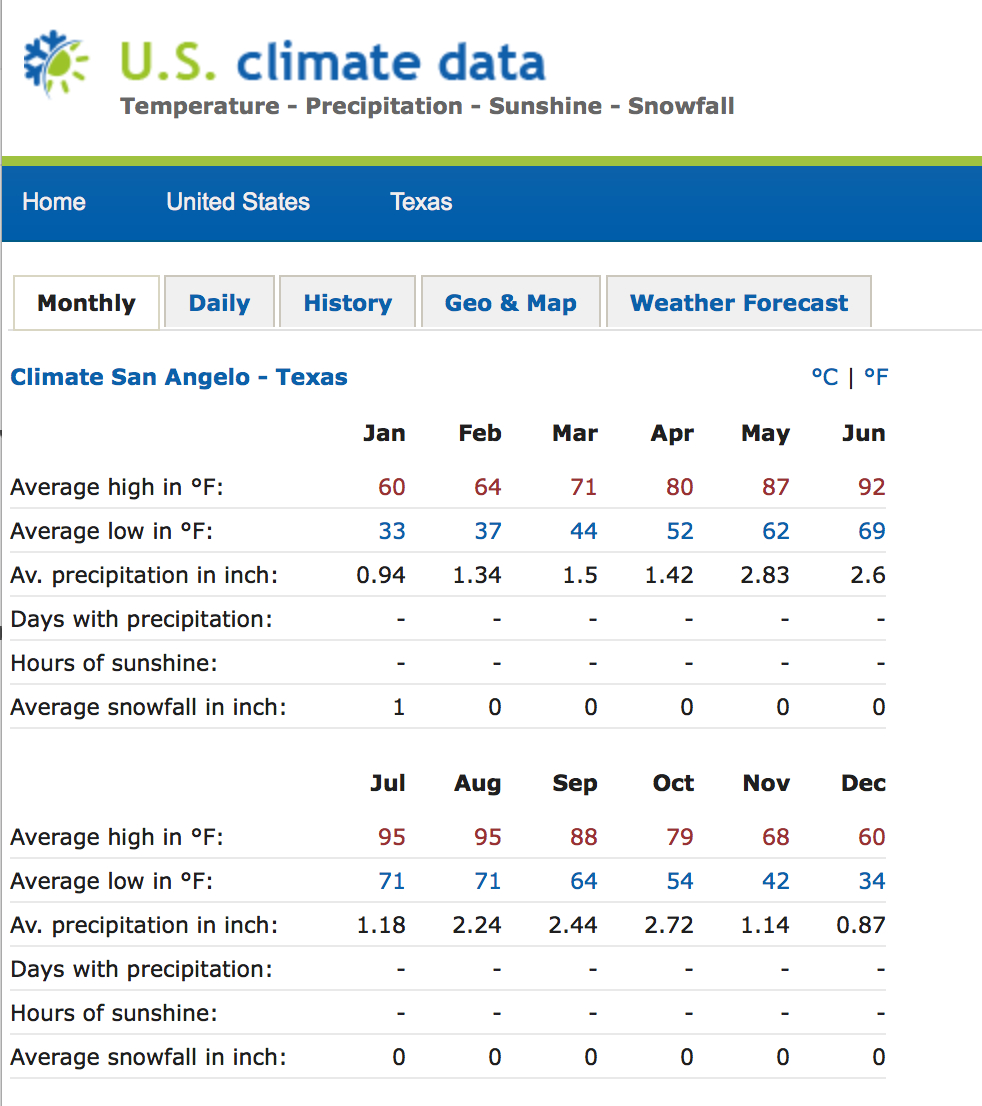
\includegraphics[width=4in]{MeanMonthlySanAngelo.jpg} 
   \caption{San Angelo climate record from Google}
   \label{fig:MeanMonthlySanAngelo}
\end{figure}

The Monthly temperature is supplied to the Blaney-Criddle Formula.   They need to be converted into Celsius.

\begin{figure}[htbp] %  figure placement: here, top, bottom, or page
   \centering
   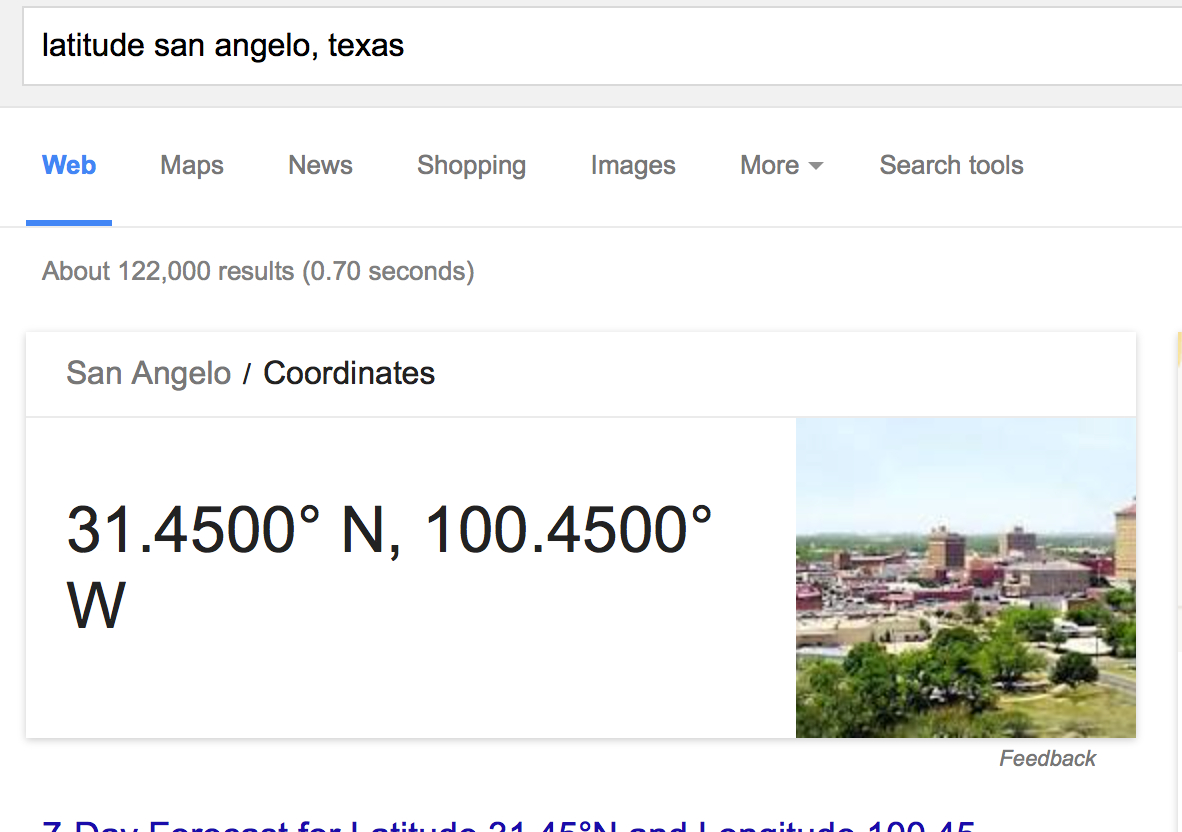
\includegraphics[width=2in]{LatitudeSanAngelo.jpg} 
   \caption{San Angelo coordinates (DDDMMSS from Google}
   \label{fig:LatitudeSanAngelo}
\end{figure}

The Latitude is also supplied to the Blaney-Criddle Formula.  We need to tell the formula we are North of the equator.

Figure \ref{fig:BlaneyCriddle} is a screen capture of the completed spreadsheet using the average of the reported high and low temperatures in Celsius reported at the website pictured in Figure \ref{fig:MeanMonthlySanAngelo}.  
\begin{figure}[h!] %  figure placement: here, top, bottom, or page
   \centering
   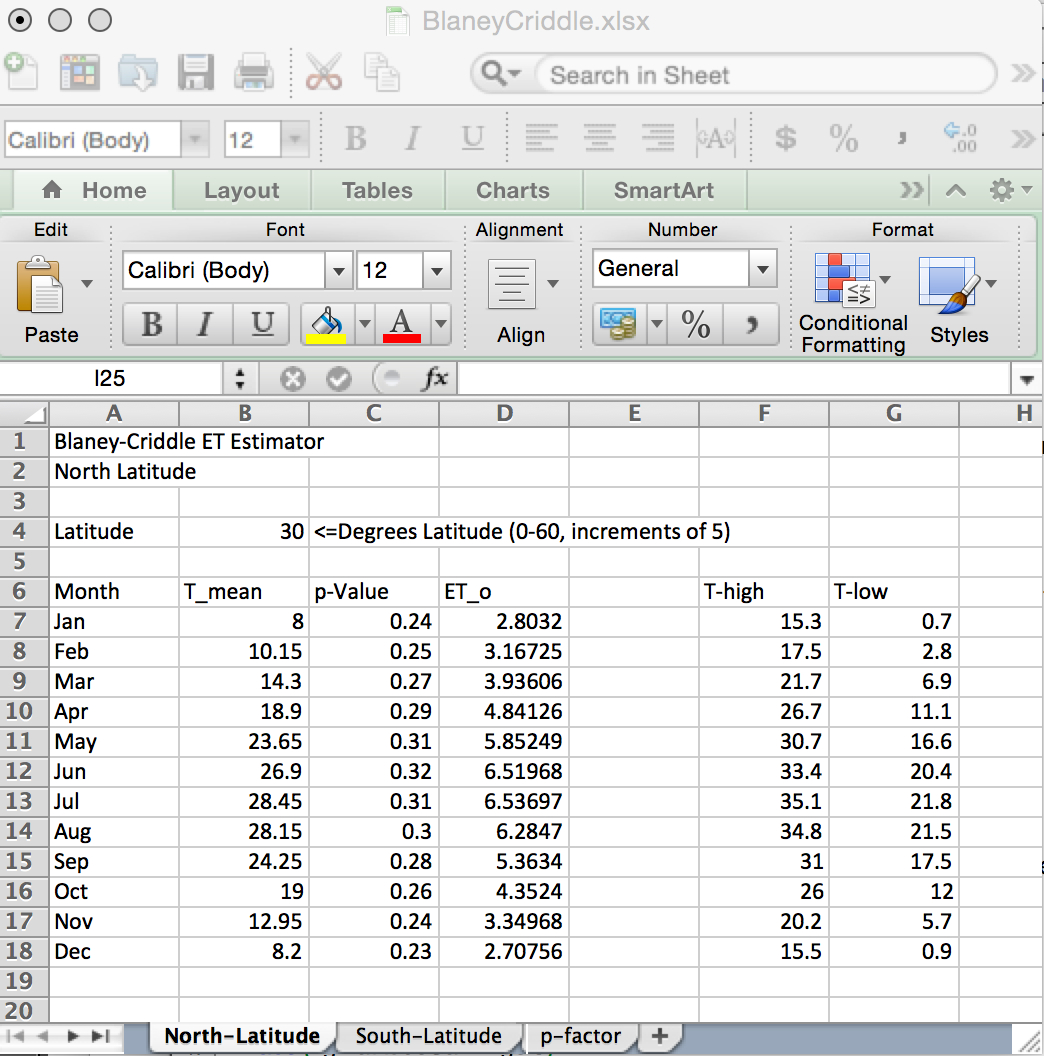
\includegraphics[width=3.5in]{BlaneyCriddle.jpg} 
   \caption{Blaney-Criddle calculations using spreadsheet supplied on class server.}
   \label{fig:BlaneyCriddle}
\end{figure}

The results indicate a high value of about 1/4 inch/day during the summer months, and about 1/10 inch per day in the winter months.

\clearpage
\item Estimate the monthly evapotranspiration depths for the San Angelo (Concho County) area using the Thornwaithe method.\footnote{A Google search should get you sufficient guidance to perform this exercise.}

\textbf{Solution}

The Thornwaite method uses the same data from the previous problem.   The Thornwaithe spreadsheet supplied on the class server is pictured in Figure \ref{fig:ThornwaitheSanAngelo}.

\begin{figure}[h!] %  figure placement: here, top, bottom, or page
   \centering
   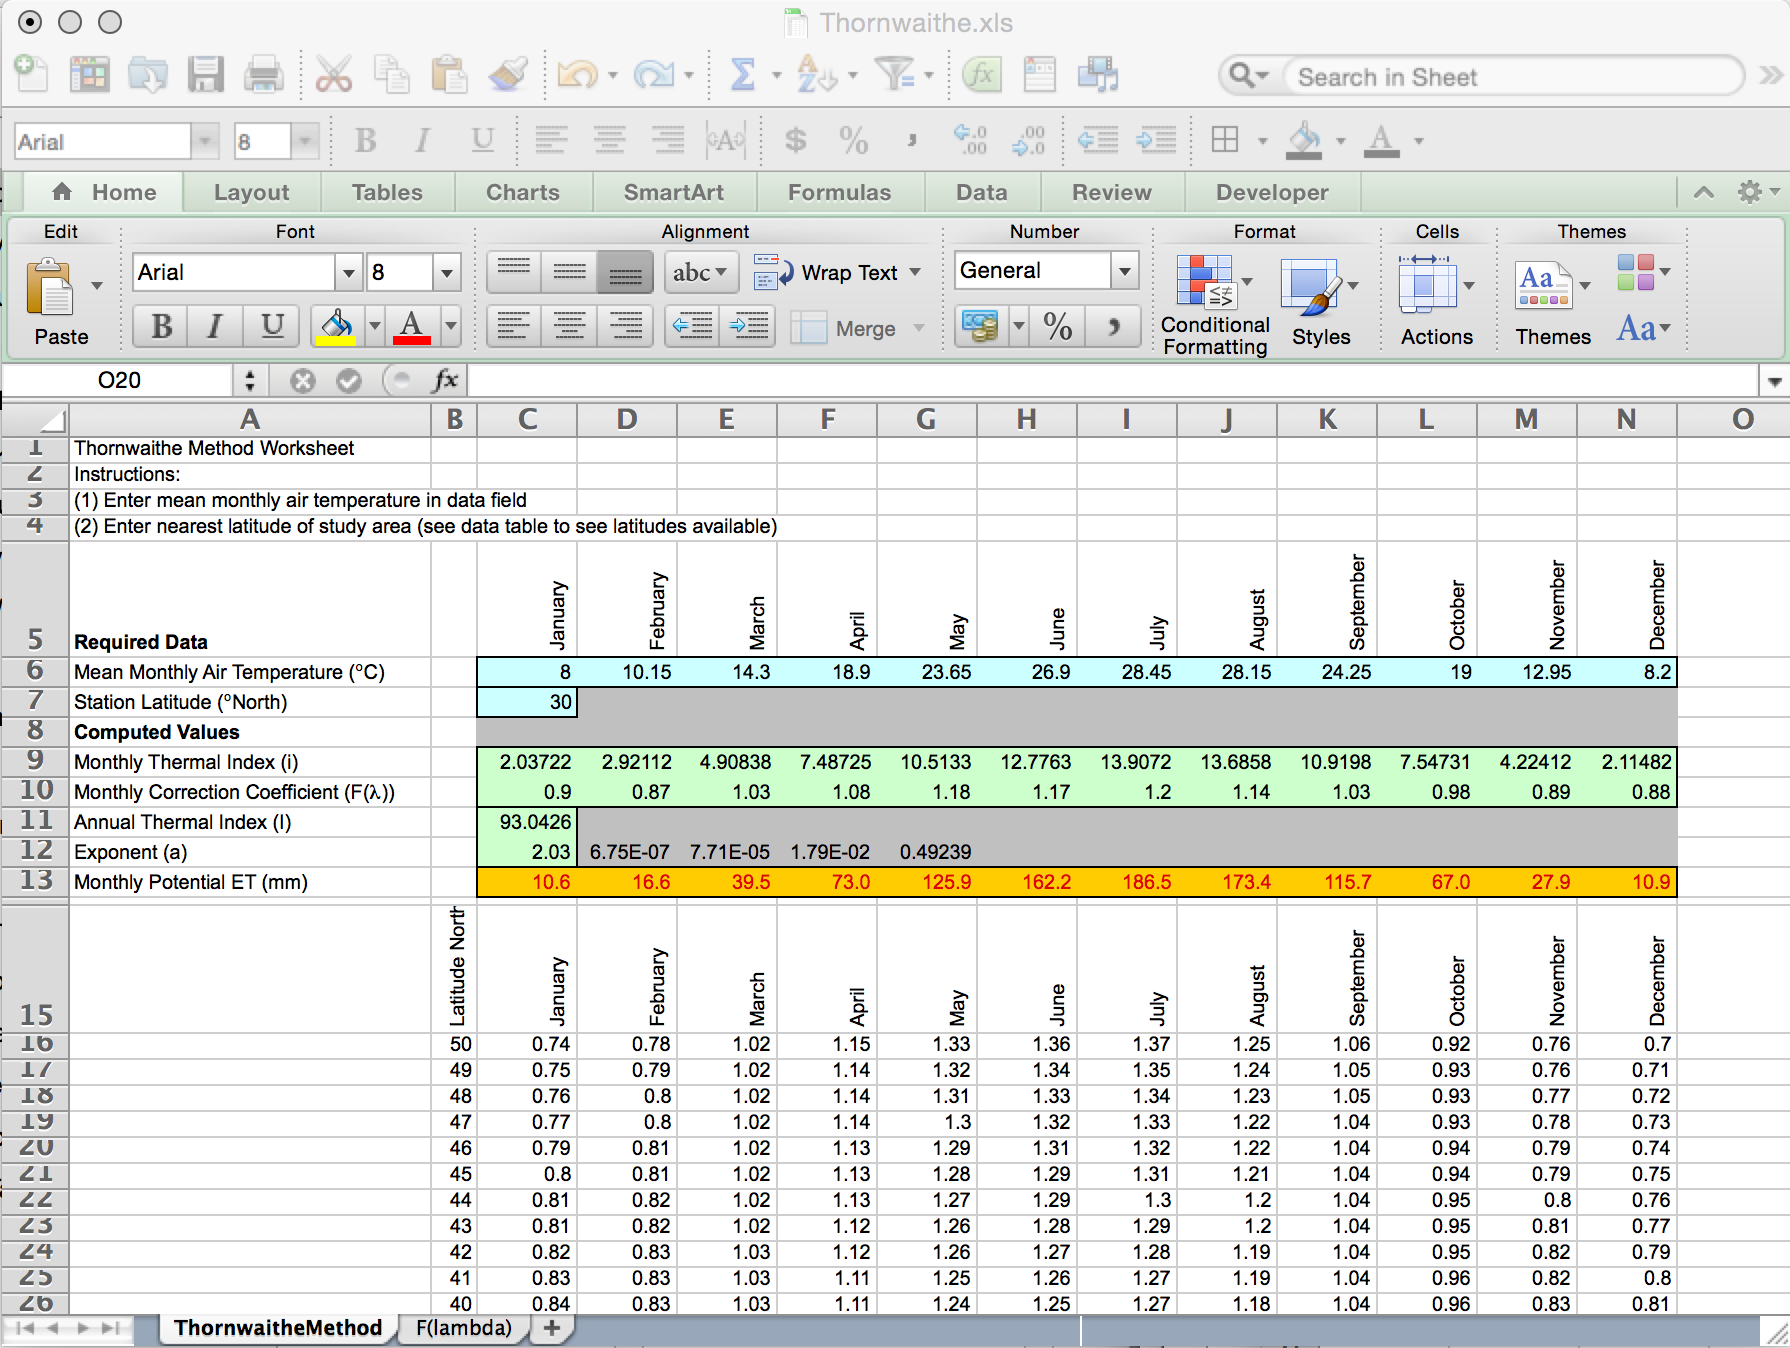
\includegraphics[width=6in]{ThornwaitheSanAngelo.jpg} 
   \caption{Thornwaithe method calculations using spreadsheet supplied on class server.}
   \label{fig:ThornwaitheSanAngelo}
\end{figure}

The results indicate a daily rate of about 1/4 inch/day  per day in the summer months and about 0.01 inches per day in the winter months.

\item How important are these estimates in the drainage analysis project for a storm lasting 24-48 hours?  Probably not terribly important for rainfall rates in excess of 1 inches per hour.   

%\item Estimate the monthly evapotranspiration depths for the Houston area using the Preistly-Taylor method\footnote{You will need to estimate the monthly evapotranspiration depths for Concho County using the Preistly-Taylor method for the semester design project.}

%\item  The file ``EVAP2.TXT'' are monthly evaporation rates for coastal Texas (from Texas Water Development Board).  Assume these are actual evaporation rates for the indicated months.  In the context of questions 2 and 3 perform the following:
%\begin{enumerate}
%\item Compare the long-term monthly averages to the rates you computed in (1) and (2).  Are they the same or different?  Any ideas why?
%\item Plot the monthly rates as a time series (the second column is the series counter).  What do you see in this plot?   Is there any trend (assuming you can remove the periodic component of the signal)?
%\item Break the data into three roughly even parts (1950-1969), (1970-1989),(1990-2009).  Perform a non-parametric hypothesis test for equal medians.  Does this data provide any evidence of a change in evaporation depth over time (that is are the median differences significant?)
%\item What would be the importance of an increase or decrease in evaporation over time (in the context of climate variability)?
%\end{enumerate}
\end{enumerate}

\end{document}  